\chapter{Introduction}  \label{Introduction}
%\section{Introduction}  \label{Introduction}

Understanding the similarities and differences of a set of source code fragments is a potentially complex problem that has many actual or potential applications in various areas of software engineering, such as detecting code clones \cite{bulychev2009evaluation}, automating source code reuse \cite{2008:fse:cottrell}, recommending replacements for APIs among various versions of a software library \cite{2014:uofc:cossette}, collating application programming interface (API) usage patterns, and automating the merge operation of various branches in a version control system. As a specific application, the focus of this study is on characterizing where logging is used in source code via the determination of structural commonalities and differences of a set of source code fragments enclosing logging calls within a software system or from different software systems.
% in program analysis, such as collating application programming interface (API) usage patterns,

Logging is a conventional programming practice of recording an application's state and/or actions during the program's execution \cite{gupta2005pro}, and log system analysis assist developers in diagnosing the presence or absence of a particular event, understanding the state of an application, and following a program's execution flow to find the root causes of an error. The importance of logging is notable in its various applications in software development and maintenance tasks such as problem diagnosis \cite{lou2010mining}, system behavioural understanding \cite{fu2013contextual}, quick debugging \cite{gupta2005pro}, performance diagnosis \cite{nagaraj2012structured}, easy software maintenance \cite{gupta2005pro}, and troubleshooting \cite{fu2009execution}.
%root causes of an error?

%Given the importance of logging, its quality can affect the quality of an application directly.
%ways, as they make different decisions
In practice, logging tasks can be performed in various ways, as developers may make different decisions about where and what to log. For example, they can apply logging to record the occurrence of every event of an application and so, they use logging calls at the start and end of the body of every method in the source code \cite{clarke1999dimension,clarke1999subject}. However, three main problems are associated with excessive logging. First, it can generate redundant information that might be confusing and misleading for developers performing system log analysis, as it masks significant information. Second, excessive logging is costly. It requires extra time and effort to write, debug, and maintain the logging code. Third, it can generate system resource overhead and thus the application performance will be negatively affected. On the other hand, insufficient logging may result in the loss of run-time information necessary for software analysis. Therefore, logging should be done in an appropriate manner to be effective.
%root causes of an error

Despite the importance of logging for software development and maintenance, few studies have been conducted on understanding logging usage in real-world applications, since logging has been considered to be a trivial task \cite{clarke1999dimension,clarke1999subject}. However, the availability of several complex frameworks (e.g., \name{log4j},\name{SLF4J}) that assist developers to log suggests that in practice effective logging is not a straightforward task to perform. In addition, a study by \citet{yuan2012characterizing} showed that developers expend great effort in modifying their logging practices as an afterthought. This indicates that it is not that simple for developers to perform logging efficiently on their first attempt.
% shows or showed?

Research on the problem of characterizing logging practices can be divided into two main topics: context and location of logging calls. The context refers to the log text messages and the location refers to where logging calls are used in the source code. A few studies have been conducted on characterizing log message modifications \cite{yuan2012characterizing} and developing tools to automatically enhance the context of existing logging calls \cite{yuan2012improving, yuan2010sherlog}. However, no research has been conducted on studying the location of logging calls in real-world software systems, though it has a great impact on the quality of logging as it helps developers to trace the code execution path to identify the root causes of an error for log system analysis. Through this research, I address this gap by developing an automated approach to detecting the detailed structural similarities and differences in the usage of logging, both within a system and between systems.


%Through this research, I would like to understand in a detailed way where developers log in practice.



% that would assist developers to make informed decisions about where and what to log
%logging has been considered as a trivial task (AOP/AOSD literature)

%\item \NZ{I am a little confused about how to find commonalities and differences of logging usage between systems? do you mean that I should compare the results taken from clustering of all Java classes in one system to another one?} \RW{The process of locating commonalities and differences can be applied within a single version of one system, across multiple versions of one system, across single versions of multiple systems, or across multiple versions of multiple systems.  It would be useful to understand the differences and similarities between different systems.  Is there some reason that this would be harder to achieve?} \NZ{I should think about it more. I can answer to this question after per-system analysis with more confidence}


\section{Programmatic support for logging} \label{background Logging}
% including or include?
A typical logging call takes parameters including a log text message and a verbosity level. A log text message consists of static text to describe the logged event and some optional variables related to the event. The verbosity level is intended to classify the severity of a logged event such as a debugging note, a minor issue, or a fatal error. Figure~\ref{fig:log-call-examples} provides examples of logging calls from the \name{log4j} framework in descending order of severity. The \name{fatal} level designates a very severe error event that will likely lead the application to terminate. The \name{error} level indicates that a non-fatal but clearly erroneous situation has occurred. The \name{warn} level indicates that the application has encountered a potentially harmful situation. The \name{info} level designates important information that might be helpful in detecting root causes of an error or in understanding the application behaviour. The \name{debug} level provides useful information for debugging an application, and it is usually used by developers only during the development phase. In general, verbosity level is used for classification, in order to avoid the overhead of creating large log files in high performance code.
% , and is usually


\begin{figure}[H]
\vspace*{1em}
\begin{center}
\begin{minipage}{3.5in}
\begin{lstlisting}[frame=single,numbers=none]
 log.fatal("Fatal Message %s", variable);
 log.error("Error Message %s", variable);
 log.warn("Warn Message %s", variable);
 log.info("Info Message %s", variable);
 log.debug("Debug Message %s", variable);
\end{lstlisting}
\end{minipage}
\caption{Logging call examples from the \protect\name{log4j} framework.\label{fig:chap1_logCode}\label{fig:log-call-examples}}
\end{center}
\end{figure}

%\RW{This isn't useful because it is too short and has already been covered by your introductory comments.}
%\section{Overview of related work} \label{intro-rw}
%
%Research on the problem of characterizing logging practices can be divided into two main topics: context and location of logging calls. The context refers to the log text messages and the location refers to where logging calls are used in the source code.
%A few studies have been conducted on characterizing log message modifications \cite{yuan2012characterizing} and developing tools to automatically enhance existing log messages \cite{yuan2012improving, yuan2010sherlog}. However, no research has been conducted on studying the location of logging calls in real-world software systems.
%
%
%Various applications have used an understanding of the commonalities and differences between source code fragments
%Understanding the commonalities and differences between source code fragments has been used for various applications (e.g., \cite{2007:esec_fse:cottrell, 2008:fse:cottrell, 2009:vissoft:cottrell, 2014:uofc:cossette, bulychev2009evaluation}). However, my study makes the first attempt to characterize the usage of logging calls by automatically detecting the detailed structural correspondences and differences of a set of  source code fragments enclosing them.



\section{Broad thesis overview} \label{intro-overview}
I aim to create an approach that provides a concise description of where logging is used in the source code by constructing generalizations that represent the detailed structural similarities and differences between entities that make logging calls, which I call \emph{logged methods} (LMs). In order to evaluate this idea, I implement the approach to operate on programs written in the Java programming language; my study investigates the location of logging calls from the point of view of logged methods. To determine how to construct generalizations using the syntax and semantics of the Java programming language, I looked to previous research conducted by \citet{2008:fse:cottrell} that determined the detailed structural correspondences between two Java source code fragments through the application of approximated anti-unification, such that one fragment can be integrated with the other one for small-scale code reuse. However, my problem context is different, as I need to generalize a set of source code fragments with special attention to logging calls. Therefore, my approach must take the logging calls into account when I perform the generalization task via the determination of structural correspondences.

%My approach employs a hierarchical clustering algorithm to create a generalization hierarchy from a set of LMs using a measure of similarity. It uses an approximated anti-unification algorithm to construct a structural generalization representing the similarities and differences between a pair of LMs. My anti-unification approach proceeds in three steps. First, it uses the Jigsaw framework \cite{2008:fse:cottrell} to determine all potential correspondences between the two LMs using a measure of similarity that relies on structural correspondences along with a simple knowledge of semantic equivalences in the Java language specifications. Second, it develops a greedy selection algorithm to approximate the best anti-unifier for my problem by determining the most similar correspondence for each substructure in my structures, applying some constraints in determining correspondences to prevent the anti-unification of logging calls with anything else. Third, it constructs an anti-unifier through the anti-unification of two structures and develops a measure of structural similarity between them.

%\RW{Your research is not about implementing a tool. Your research is about developing an approach, a concept, which you then implement in order to perform experiments.  The concept does not depend on Java, or the JDT, or Jigsaw: these are implementation-level choices.  If your implementation contains bugs, this does not immediately reflect on the concept.  If the concept has bugs, this will be reflected in the implementation.}
My approach to characterizing logging usage proceeds in four steps (as shown in Figure~\ref{fig:system_overview}). First, potential structural correspondences are determined between the abstract syntax trees (ASTs) of LMs in a pairwise manner, and stored in a novel structure: the \emph{anti-unifier AST} (AUAST), which allows the application of anti-unification on AST structures. Second, I use an approximated anti-unification algorithm to construct a structural generalization (an anti-unifier) representing the commonalities and differences between AUAST pairs, which employs a greedy selection algorithm to approximate the best anti-unifier for the problem by determining the most similar correspondence for each node. The anti-unification algorithm applies some constraints prior to determining the best correspondences, in order to prevent the anti-unification of logging calls with any other type of nodes in the tree structure. The anti-unifier is constructed through the anti-unification of each AUAST node with its best correspondences and then a measure of structural similarity is developed between the two AUASTs. 
%The first two steps are described in Chapter~\ref{methodology}.
In the third step, I employ a hierarchical clustering algorithm to group the AUASTs into clusters using the structural similarity measure and I then create a structural generalization from each cluster. %This step is realized by my clustering tool (Chapter~\ref{clustering}).
The last step involves analyzing the structural generalizations to extract logging usage schemas that represent the structural commonalities of the set of LMs within each cluster.
%create a generalization hierarchy from a set of LMs using a measure of similarity.

To evaluate the approach, I implemented it in a tool written in the Java programming language. I use the Eclipse JDT framework to extract the AST of LMs from a Java program, and employ the Jigsaw framework developed by \citet{2008:fse:cottrell} to find potential structural correspondences. My anti-unifier building tool (built atop Jigsaw) is applied to construct a detailed view of structural generalizations (Section~\ref{antiunifierTool}), and my clustering tool is developed atop of it to perform the clustering algorithm described in Section~\ref{clustering-alg}. 
%atop the anti-unifier building tool

%My correspondence tool (Section~\ref{corr-tool}) is employed to create AUASTs, and

%use the Jigsaw framework that relies on structural correspondences along with a simple knowledge of semantic equivalences in the Java language specifications to determine potential correspondence connections between AUASTs of the two LMs and measure the similarity between the nodes involved in each connection.


\begin{figure} [t]
  \centering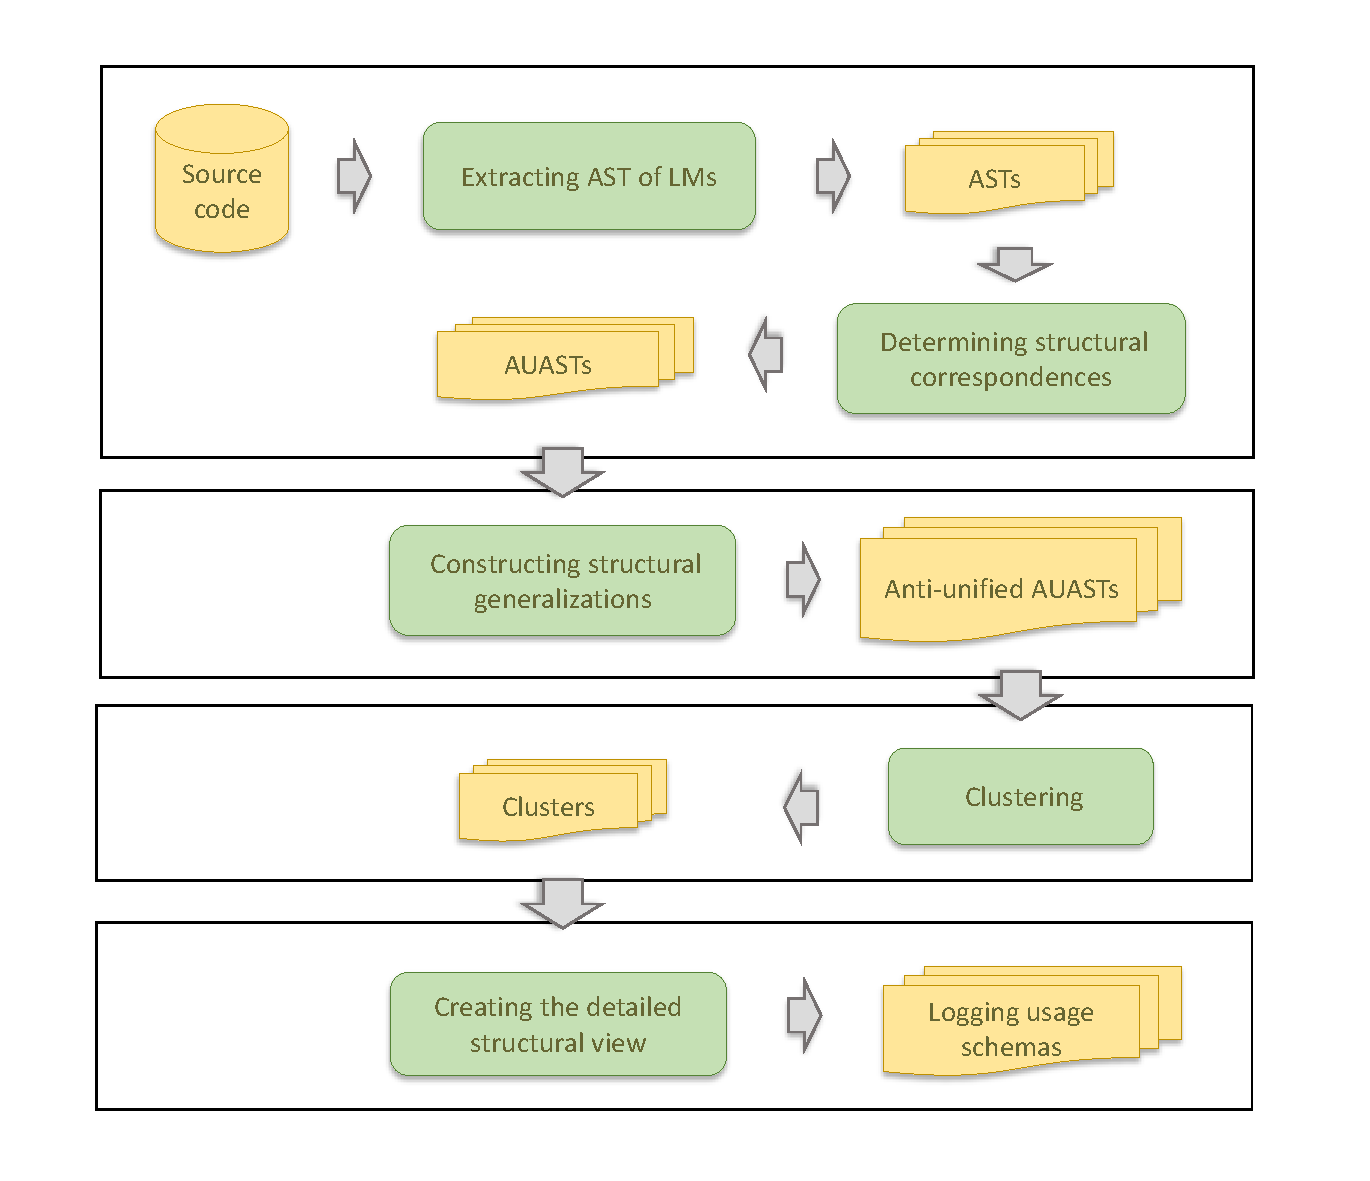
\includegraphics [width = \textwidth]{Drawing4/SystemOverview.pdf}
  \caption{Overview of the approach. %\protect\RW{I don't want to see mention of tools here.  This should be focused on the concepts.}
  }
  \label{fig:system_overview}
\end{figure}

%most similar  or best correspondence?
%constraints wording?
%my emprical study?
%My tool has been applied on the source code of these systems and extracts all logged Java methods from these systems to construct the structural generalizations.
%My evaluation shows ...

\section{Thesis statement} \label{intro-stmt}
The thesis of this work is that the detailed structural similarities and differences between source code that makes use of logging calls can be determined via higher-order anti-unification modulo theories, providing a concise and accurate description of where logging calls do occur in real-world software systems.
%via HOAUMT and clustering???

\section{Thesis organization} \label{intro-org}
The remainder of the thesis is organized as follows.

Chapter~\ref{ch2} motivates the problem of understanding where to use logging calls in source code through a scenario in which a developer attempts to perform a logging task. This scenario outlines the potential problems she may encounter and illustrates that the current logging practice is insufficiently supported.

Chapter~\ref{background} provides background information that I build atop: abstract syntax trees (ASTs), which are the basic structure I will use for describing software source code; the Eclipse JDT, an industrial framework for producing and manipulating ASTs for source code written in the Java programming language; anti-unification, which is a theoretical approach for determining similarities and differences in tree structures; and on Jigsaw, a research tool based on the Eclipse JDT for performing anti-unification.

Chapters~\ref{background2},~\ref{methodology}, and~\ref{clustering} present the first three steps of my approach. Determining structural correspondences between AUASTs; constructing structural generalizations from an AUAST pair; and classifying a set of AUASTs into separate clusters, respectively. In each chapter, I discuss the implementation of my approach as an Eclipse plug-in, and conduct an experimental study to assess the effectiveness of my approach through the application of its tool support on a sample test suite extracted from a real software system.



Chapter~\ref{eval} presents an empirical study I conducted to characterize the location of logging usage in three open-source software systems. Chapter~\ref{diss} discusses the results and findings of my work, threats to its validity, and remaining issues. Chapter~\ref{rw} describes work related to my research problem and how it does not adequately address the problem. Chapter~\ref{conc} concludes the dissertation and presents the contributions of this study and future work. %Additional materials appended this dissertation are provided in Appendix A.


% difference between experimental or empirical study


